%%%%%%%%%%%%%%% Page Setup %%%%%%%%%%%%%%%

\documentclass[a4paper, 11pt]{book}
\usepackage[utf8]{inputenc}
\usepackage[framemethod=tikz]{mdframed}
\usepackage[margin=3cm]{geometry}
\setlength\parindent{0pt}
\setlength{\parskip}{\baselineskip}%
\usepackage{graphicx}
\usepackage{tgadventor}
%\renewcommand*\familydefault{\sfdefault}
\usepackage[T1]{fontenc}
\usepackage{bm}

%%%%%%%%%%%%%%% Math Stuff %%%%%%%%%%%%%%%

\usepackage{amsmath}
\usepackage{amssymb}
\usepackage{tikz}
\usepackage{tikz-cd}
\usepackage{tkz-euclide}
\usepackage{pgf-pie}
\usepackage{cancel}

%%%%%%%%%%%%%%% Quotation Stuff %%%%%%%%%%%%%%%

\usepackage[english]{babel}
\usepackage[autostyle]{csquotes}

%%%%%%%%%%%%%%% Color %%%%%%%%%%%%%%%

\definecolor{p}{rgb}{0.9118, 0.4961, 0.6804}
\definecolor{p1}{rgb}{1, 0.92, 0.963}
\definecolor{g}{rgb}{0.023, 0.477, 0.219}
\definecolor{g1}{rgb}{0.03, 0.75, 0.20}
\definecolor{g2}{rgb}{0.95, 1, 0.95}

%%%%%%%%%%%%%%% Link Setup %%%%%%%%%%%%%%%

\usepackage{hyperref}
\hypersetup{colorlinks=true, linkcolor=g, filecolor=g, urlcolor=g,}

%%%%%%%%%%%%%%% Box %%%%%%%%%%%%%%%

\newmdenv[innerlinewidth=2pt, roundcorner=4pt,linecolor=g1,innerleftmargin=20pt,
innerrightmargin=20pt,innertopmargin=20pt,innerbottommargin=20pt,backgroundcolor = g2]{mybox}

%%%%%%%%%%%%%%% Border Stuff %%%%%%%%%%%%%%%

\usepackage{fancyhdr}
\pagestyle{fancy}
\fancyhf{}
\fancyhead[LE,RO]{\leftmark}
\fancyhead[RE,LO]{\thepage}
\fancyfoot[CE,CO]{}
\fancyfoot[LE,RO]{}

%%%%%%%%%%%%%%% Bug Fix Adjustments %%%%%%%%%%%%%%%

\setlength{\headheight}{14pt}
\setlength{\footskip}{55pt}

%%%%%%%%%%%%%%% Index %%%%%%%%%%%%%%%

\usepackage{makeidx}
\makeindex

%%%%%%%%%%%%%%% Custom Commands %%%%%%%%%%%%%%%

\def\greenlozenge{\mathbin{\color{g}\blacklozenge}}

\newcommand{\emphasis}[1]{\underline{\textbf{#1}} }
\newcommand{\vocab}[1]{\underline{\textbf{#1}}\index{#1}}

\newcommand{\claim}{\textbf{\underline{Claim}} }
%\newcommand{\corollary}{\underline{\textbf{Corollary}} }
\newcommand{\defn}{\underline{\textbf{Def}} }
\newcommand{\digression}{\underline{\textbf{Digression}} }
\newcommand{\easy}{\underline{\textbf{Easy}} }
\newcommand{\example}{\underline{\textbf{Example}} }
\newcommand{\fact}{\underline{\textbf{Fact}} }
\newcommand{\facts}{\underline{\textbf{Facts}} }
\newcommand{\goal}{\underline{\textbf{Goal}} }
\newcommand{\idea}{\underline{\textbf{Idea}} }
%\newcommand{\lemma}{\underline{\textbf{Lemma}} }
\newcommand{\need}{\underline{\textbf{Need}} }
\newcommand{\note}{\underline{\textbf{Note}} }
\newcommand{\proof}{\underline{\textbf{Proof}} }
\newcommand{\recall}{\underline{\textbf{Recall}} }
\newcommand{\remark}{\underline{\textbf{Remark}} }
%\newcommand{\theorem}{\underline{\textbf{Theorem}} }
\newcommand{\verify}{\underline{\textbf{Verify}} }


%%%%%%%%%%%%%%% New Theorems %%%%%%%%%%%%%%%


\newtheorem{theorem}{Theorem}[section]
\newtheorem{corollary}{Corollary}[theorem]
\newtheorem{lemma}[theorem]{Lemma}
\newtheorem{conjecture}[theorem]{Conjecture}

%%%%%%%%%%%%%%% Math Operators %%%%%%%%%%%%%%%
\DeclareMathOperator{\A}{\mathbb{A}}
\DeclareMathOperator{\Aut}{Aut}
\DeclareMathOperator{\C}{\mathbb{C}}
\DeclareMathOperator{\characteristic}{char}
\DeclareMathOperator{\cod}{cod}
\DeclareMathOperator{\dom}{dom}
\DeclareMathOperator{\Fix}{Fix}
\DeclareMathOperator{\Frac}{Frac}
\DeclareMathOperator{\Free}{Free}
\DeclareMathOperator{\id}{id}
\DeclareMathOperator{\Ima}{Im}
\DeclareMathOperator{\Mor}{Mor}
\DeclareMathOperator{\N}{\mathbb{N}}
\DeclareMathOperator{\Obj}{Obj}
\DeclareMathOperator{\Q}{\mathbb{Q}}
\DeclareMathOperator{\R}{\mathbb{R}}
\DeclareMathOperator{\Res}{Res}
\DeclareMathOperator{\Stab}{Stab}
\DeclareMathOperator{\Span}{span}
\DeclareMathOperator{\Spec}{Spec}
\DeclareMathOperator{\Z}{\mathbb{Z}}
%%%%%%%%%%%%%%% Title %%%%%%%%%%%%%%%

\title{Transcendental Numbers (Draft)}
\author{Vincent Lin}
\date{Last Updated: \today}


\begin{document}
\frontmatter
\maketitle
\tableofcontents
\chapter{Preface}
This uses the background information from 21441 and algebra and reviews it in order to discuss transcendental numbers. Then, it will introduce methods of explicitly constructing, finding, and detecting transcendental numbers. Several classes of transcendental numbers will be named and the methods of finding them will be discussed, including the Lindemann-Weierstrass theorem, Gelfond-Schneider theorem, and Baker's theorem. It concludes with a discussion of Schanuel's conjecture. The main sequence of theorems is primarily related to determining the transcendence of complex numbers using auxiliary functions, but there are many ways of finding transcendental numbers.
\mainmatter{}
\chapter{Preliminaries}
\section{Algebraic and Transcendental Numbers}

\defn{An \vocab{algebraic number} is $\alpha \in \C$ which is the root of a nonzero polynomial in $\Q[x]$. A \vocab{transcendental number} is a complex number that is not algebraic.}\par

\note{We will use $\A$ to denote the set of algebraic numbers and we will use $\C \setminus \A$ to denote the set transcendental numbers. We will use $\R \setminus \A$ to denote the set of real transcendental numbers.}\par

To find examples of algebraic numbers, we can take any nonzero polynomial in $\Q[x]$ find its roots. By definition, these roots are algebraic numbers. For example, $\sqrt{2}$ is algebraic because it is a root of $x^2 - 2$. Also, $i$ is algebraic because it is the root of $x^2 + 1$. All rational numbers are algebraic as well. Let $\frac{p}{q} \in \Q$ be rational, where $p, q \in \Z$ and $q$ is nonzero. Then, it is the root of $x - \frac{p}{q}$. Therefore, $\Q \subseteq \A$.\par

What about transcendental numbers? Do they exist?\par

\begin{mybox}
    \theorem{Yes, transcendental numbers exist.}
\end{mybox}

\proof{Consider the set of algebraic numbers, which we will denote by $\A$. This set is countable. We will show this by forming a surjection  \[\phi : \left(\N \times \bigcup\limits_{n \in \N} \Q^{n}\right) \to \A.\] Note that $\N \times \bigcup\limits_{n \in \N} {\Q}^{n}$ is countable because it is the Cartesian product of a countable set with a countable union of countable sets. By the fundamental theorem of algebra, we know that a polynomial of degree $k$ has $k$ (not necessarily distinct) roots. Therefore, we can number the $k$ roots from $1$ to $k$ for each polynomial. Thus, if we specify the nonzero rational coefficients $(a_0, \ldots, a_k)$ and an index $i$ for $i \in [k]$ to be the $i$-th root of the polynomial $a_k x^k + \cdots + a_0$, we get an algebraic number. We define the map $\phi(i, (a_0, \ldots, a_k))$ to be the $i$-th root of $a_k x^k + \cdots + a_0$ if it exists. Otherwise, we map the input to zero. From the definition, we know that every algebraic number can be encoded this way since it is one of the roots of a nonzero rational polynomial. Thus, for all $a \in \A$, there must be an input $x$ such that $\phi(x) = a$, making this a surjective map from a countable set to $\A$. This makes $\A$ countable. However, since $\C$ is uncountable, it cannot be the case that all complex numbers are algebraic. Thus, if a complex number is not algebraic, it must be transcendental. Furthermore, $\R$ is uncountable so there must be real transcendental numbers as well.\[ \greenlozenge \]}

If transcendental numbers exist, then can we find an example? To show that a number is algebraic, we just have to find a nonzero rational polynomial that it is a root of, evaluate that polynomial at that number, and verify that we get zero. However, checking if a number is transcendental is a very hard problem. The rest of this paper will discuss the transcendence of a large class of numbers and methods for determining transcendence.\par

\section{Algebra Preliminaries}

Before that, we will generalize the concept of transcendence to other fields. In order to do this, we will list several definitions. Let $K, L$ be fields and let $L/K$ be a field extension. We will introduce a few definitions for recall.\par

\recall{\begin{itemize}
    \item{$a \in L$ is \vocab{algebraic} over $K$ if there is a nonzero polynomial $f \in K[x]$ such that $f(a) = 0$. Otherwise, $a$ is \vocab{transcendental} over $K$. In other words, an algebraic number is a complex number that is algebraic over $\Q$ and a transcendental number is a complex number that is not algebraic over $\Q$.} 
    \item{$X \subseteq L$ is \vocab{algebraically independent} over $K$ if for all $a_1, \ldots, a_t$ distinct and all $f \in K[x_1, \ldots, x_t]$, $f(a_1, \ldots, a_t) = 0$ implies $f = 0$.}
    \item{If $a \in L$ is algebraic over $K$, the \vocab{minimal polynomial} of $a$ over $K$, denoted $m^K_a$ or $m_a$ when the underlying field is implied, is the unique monic irreducible polynomial which generates the kernel of the evaluation map $\phi(f) = f(a)$ for $f \in K[x]$. The \vocab{degree} of $\alpha \in K$ is the degree of the minimial polynomial $m_a$ and the \vocab{conjugates} of $a$ are the roots of $m_a$.}
    \item{$L/K$ is an \vocab{algebraic extension} if every element in $L$ is algebraic over $K$.}
    \item{$L$ is \vocab{algebraically closed} if every nonconstant single variable polynomial in $L$ has a root in $L$.}
    \item{An \vocab{algebraic closure} of $K$ is an algebraic extension of $K$ that is algebraically closed.}
    \end{itemize}}
\par
Now we will consider some important facts about number fields:\par
\recall{\begin{itemize}
    \item{An \vocab{algebraic number field} or \vocab{number field} is an algebraic extension of $\Q$.}
    \item{An \vocab{algebraic integer} is $\alpha \in \C$ such that it is the root of a monic polynomial in $\Z[x]$.}
    \item{If $K$ is a number field, $\mathcal{O}_K$ is the \vocab{ring of integers} of $K$ and is the ring of all algebraic integers in $K$. It is a free $\Z$-module of rank $[K : \Q]$. If $\alpha \in K$, there is a positive $c \in \Z$ such that $c\alpha \in \mathcal{O}_K$.}
    \item{Let $K$ be a number field. An \vocab{integral basis} is a $\Q$-basis for $K$ that is also a $\Z$-basis for $\mathcal{O}_K$.}
    \end{itemize}}

\begin{mybox}
    \lemma{Let $K$ be a number field and let $\alpha \in K$. The degree of $\alpha$ over $\Q$ divides the degree of $K$.\par}
\end{mybox}
\proof{By the tower law, $[K : \Q(\alpha)][\Q(\alpha) : \Q] = [K:\Q]$. Thus, $[\Q(\alpha):\Q] \mid [K:\Q]$.\par\[\greenlozenge\]}


\note{Let $K$ be a number field of degree $n$ over $\Q$ and let $\alpha \in K$. Then, let $\sigma_1, \ldots, \sigma_n$ be the $\Q$-fixing embeddings $K \hookrightarrow \C$. We write $\| \alpha \|$ to denote $\max\limits_{i \in \{1, \ldots ,n\}} \vert \sigma_i(\alpha) \vert$.\par}

\begin{mybox}
    \lemma{Let $\alpha, \beta \in K$, a number field. Then, $\|\alpha + \beta\| \leq \| \alpha \| + \| \beta \|$ and $\| \alpha\beta \| \leq \| \alpha \| \| \beta \|$.}
\end{mybox}

\proof{We first show this for addition. 
    \begin{align*}\| \alpha + \beta \| &= \max\limits_{i \in \{1, \ldots, n\}} \vert \sigma_i(\alpha + \beta) \vert \\ &= \max\limits_{i \in \{1, \ldots, n\}} \vert \sigma_i(\alpha) + \sigma_i(\beta) \vert \\ &\leq \max\limits_{i \in \{1, \ldots, n\}} \vert \sigma_i(\alpha) \vert + \vert \sigma_i(\beta) \vert \\ &\leq \max\limits_{i \in \{1, \ldots, n\}} \vert \sigma_i(\alpha) \vert + \max\limits_{i \in \{1, \ldots, n\}} \vert \sigma_i(\beta) \vert \\ &= \| \alpha \| + \| \beta \| \end{align*} 
The proof for multiplication is similar by replacing $+$ with $\cdot$ instead.\[ \greenlozenge \]}
\begin{mybox}
    \lemma{If $K$ is a number field, it has an integral basis.\par}
\end{mybox}
\proof{We know that $\mathcal{O}_K$ is a free $\Z$-module of rank $n := [K : \Q]$ so let $\{\beta_1, \ldots, \beta_n\}$ be a basis for $\mathcal{O}_K$ as a $\Z$-module. To show that this is a basis for $K$, we will show that this set $\Q$-spans $K$ and is $\Q$-linearly independent.\par

First, we will show it is spanning. Let $\alpha \in K$. Then, find positive $c \in \Z$  such that $c\alpha \in \mathcal{O}_K$. Now, for $\lambda_1, \ldots, \lambda_n \in \Z$, we can write \[c\alpha = \lambda_1 \beta_1 + \cdots + \lambda_n \beta_n.\] Therefore, since $c > 0$, and is an integer, we can divide by $c$ to get \[\alpha = \frac{\lambda_1}{c} \beta_1 + \cdots + \frac{\lambda_n}{c} \beta_n.\] Since $\frac{\lambda_i}{c} \in \Q$, we know that the basis $\Q$-spans $K$. Now, we will show it is $\Q$-linearly independent. Suppose for contradiction \[0 = \lambda_1\beta_1 + \cdots + \lambda_n\beta_n,\] where $\lambda_i \in \Q$ but there is a nonzero $\lambda_i$. Then, we can multiply both sides by the least common multiple of the demoninators of the $\lambda_i$ to get that the $\lambda_i$'s are not $\Z$-linearly independent, which is a contradiction.\par \[ \greenlozenge \]}

\newpage
\begin{mybox}
    \lemma{For any nonzero polynomial $p(x) \in \C[x]$ with a root at $x = \alpha$ of multiplicity $m > 0$, $p'(x)$, has the root $\alpha$ with multiplicity $m-1$. More generally, if $R$ is an integral domain and $p \in R[x]$ has $\alpha$ with multiplicity $m$, $p'$, the formal derivative, has root $\alpha$ with multiplicity $m-1$ if $\characteristic (R)$ is not a factor of $m$.}
\end{mybox}

\proof{We can write $p(x)$ as ${(x-\alpha)}^{m}q(x)$ where $(x-\alpha) \nmid q(x)$. Now, taking the derivatives of both sides and using the product rule, we get
\begin{align*}
    p(x) &= {(x-\alpha)}^{m}q(x) \\
    p'(x) &= \left({(x-\alpha)}^{m}\right)'q(x) + {(x-\alpha)}^{m}q'(x) \\
          &= m{\left(x- \alpha\right)}^{m-1}q(x) + {(x-\alpha)}^{m}q'(x) \\
          &= {\left(x-\alpha\right)}^{m-1}\left(mq(x) + (x-\alpha)q'(x)\right)
\end{align*}

Therefore, we get that ${(x-\alpha)}^{m-1} \mid p'(x)$ so $p'(x)$ has the root $\alpha$ of multiplicity at least $m-1$.\par


Now, we want to show that $p'(x)$ has root $\alpha$ with multiplicity at most $m-1$. We need to show that $x-\alpha$ does not divide $\left(mq(x) + (x-\alpha)q'(x)\right)$. We can take this expression modulo $(x-\alpha)$ to get that it is equivalent to $mq(x)$. Note that $(x-\alpha) \nmid q(x)$, so we need $m > 0$. This is true when $\characteristic(R)$ is not a factor of $m$ (otherwise the entire expression is zero). Therefore, we have multiplicity at most $m-1$. Since $\characteristic(\C) = 0$, we know this rule applies to complex polynomials.\par
\[ \greenlozenge \]}


\defn{The square \vocab{Vandermonde matrix} of size $n$ is the matrix $V = V(x_1, \ldots, x_n)$ is the $n \times n$ matrix 
\[
    \begin{pmatrix}
        1 & x_1 & x_{1}^2 & \cdots & x_{1}^{n-1} \\
        1 & x_2 & x_{2}^2 & \cdots & x_{2}^{n-1} \\
        1 & x_3 & x_{3}^2 & \cdots & x_{3}^{n-1} \\
        \vdots & \vdots & \vdots & \ddots & \vdots \\
        1 & x_n & x_{n}^2 & \cdots & x_{n}^{n-1}
    \end{pmatrix}
\]
}
with nonzero complex elements $x_i^{j}$ in the $i$-th row and $j+1$-th column column where $0 \leq j \leq n-1$ and $1 \leq i \leq n$.\par
\newpage
\begin{mybox}
    \lemma{Let $V = V(x_1, \ldots, x_n)$ be the square Vandermonde matrix of size $n$. Then, the determinant of the square Vandermonde matrix is \[\prod\limits_{1 \leq i < j \leq n} (x_j - x_i).\] Therefore, the determinant vanishes if and only if $x_i = x_j$ for any $i \neq j$.} 
\end{mybox}

\proof{For $1 \leq i \leq n$, let $E := {\{e_i\}}$ be the canonical basis for ${\C}^{n}$.\par

    Let $P_n$ be the $\C$-vector space of polynomials with degree less than $n$. Furthermore, for $1 \leq i \leq n$, let $A := \{a_i\}$ be the monomial basis for $P_n$ where $a_i(x) = x^{i-1}$ and let $B := \{b_i\}$ be another monomial basis for $P_n$ where $b_i(x) = \prod\limits_{j < i} (x-x_j)$. For example, 
\begin{align*}
    b_1 &= 1, \\ 
    b_2 &= (x - x_1), \\ 
    b_3 &= (x - x_1)(x - x_2), \\
        &\vdots \\
    b_n &= (x - x_1)(x - x_2) \ldots (x - x_{n-1}).
\end{align*}
Consider the linear transformation $\psi : P_n \to \C^n$ via $\psi(p) = (p(x_1), \ldots, p(x_n))$. We can think of this as a map from $p(x)$ to a column vector of length $n$. 
\[
    p \mapsto 
    \begin{pmatrix}
        p(x_1) \\
        p(x_2) \\
        \vdots \\
        p(x_n)
    \end{pmatrix}
\]
Let $V$ be the matrix of $\psi$ with respect to $A$ and $E$. Now, let $L$ be the matrix of $\psi$ with respect to $B$ and $E$. Finally, let $U$ be the change of basis matrix from $B$ to $A$. Then, 
\begin{align*}
    &VU = L \\
    &\det(VU) = \det(L) \\
    &\det(V)\det(U) = \det(L)
\end{align*}

Now, $V$, the matrix of $\psi$ with respect to $A$ and $E$ is  
\[\begin{pmatrix}
    \vert & \vert &\cdots & \vert \\
    \psi(a_1) & \psi(a_2) &\cdots & \psi(a_n) \\
    \vert & \vert &\cdots & \vert
\end{pmatrix} = 
\begin{pmatrix}
    1 & x_1 & \cdots & x_1^{n-1} \\
    1 & x_2 & \cdots & x_2^{n-1} \\
    \vdots & \vdots & \ddots & \vdots \\
    1 & x_n & \cdots & x_n^{n-1}
\end{pmatrix},\] 
the square Vandermonde matrix of size $n$.\par

On the other hand, $L$, the matrix of $\psi$ with respect to $B$ and $E$ is
\[\begin{pmatrix}
    \vert & \vert &\cdots & \vert \\
    \psi(b_1) & \psi(b_2) &\cdots & \psi(b_n) \\
    \vert & \vert &\cdots & \vert
\end{pmatrix}
\]
\[
= \begin{pmatrix}
    1 & \textcolor{red}{\cancelto{0}{(x_1-x_1)}}&\cdots & \textcolor{red}{\cancelto{0}{(x_1-x_1)}}(x_1-x_2)\ldots (x_1-x_{n-1}) \\
    1 & (x_2-x_1) &\cdots & (x_2-x_1)\textcolor{red}{\cancelto{0}{(x_2-x_2)}}\ldots (x_2-x_{n-1}) \\
    \vdots & \vdots &\ddots & \vdots \\
    1 & (x_n-x_1) & \cdots& (x_n-x_1)(x_n-x_2)\ldots(x_n-x_{n-1})
\end{pmatrix} 
\]
\[
=  \begin{pmatrix}
    1 &  0 &\cdots & 0 \\
    1 & (x_2-x_1) & \cdots & 0 \\
    \vdots & \vdots &\ddots & \vdots \\
    1 & (x_n-x_1) & \cdots& (x_n-x_1)(x_n-x_2)\ldots(x_n-x_{n-1})
\end{pmatrix} 
\]
Note that $L$ is lower triangular so $\det(L)$ is the product of the entries along its diagonal, or $\prod\limits_{1 \leq i < j \leq n} (x_j - x_i)$.\par

Finally, consider the change of basis matrix $U$ from basis $B$ to basis $A$ in $P_n$. The columns of $U$ records the coefficients of the $b_i$ polynomials after expanding. Note that since the $b_i$ are monic, the diagonal of $U$ consists of all $1$s because the $(i,i)$-entry of $U$ is the coefficient of $x^{i-1}$ (the leading coefficient) in $b_i$. Therefore, $U$ is of the form

\[
    \begin{pmatrix}
        1 & \text{blah} & \text{blah} & \cdots & \text{blah} \\
        0 & 1           & \text{blah} & \cdots & \text{blah} \\
        0 & 0           & 1           & \cdots & \text{blah} \\
        \vdots & \vdots  & \vdots & \ddots & \vdots \\
        0 & 0 & 0 & \cdots & 1
    \end{pmatrix}.
\]
Thus, since $U$ is upper triangular, $\det(U)$ is the product of the $1$s along the diagonal so $\det(U) = 1$.\par

Plugging what we know about $\det(L)$ and $\det(U)$ into $\det(V)\det(U) = \det(L)$, we get that $\det(V) = \prod\limits_{1 \leq i < j \leq n} (x_j - x_i)$.

\[\greenlozenge\]
}

\section{Analysis Preliminaries}
Now we will introduce some concepts from complex analysis. Consider the set of complex numbers $\C$ as a normed space equipped with the absolute value function $\vert \cdot \vert : \C \to \R$ via $\vert z \vert = \sqrt{z\bar{z}}$, where $\bar{z}$ is the complex conjugate of $z$. This norm induces a metric space, so we can define the distance between $x$ and $y$ as $d(x,y) := \vert x - y \vert$. Furthermore, this metric space induces a topological space so we can define open sets $U \subseteq \C$ such that all points $z \in U$ are contained in a ball within $U$ centered at $z$. In other words, for all $z \in U$, there is $\varepsilon > 0$ such that for all $y$ where $d(z,y) < \varepsilon$, $y \in U$.\par

\defn{Let $f : \C \to \C$ be a function. The \vocab{limit} of $f$ as $z \to z_0$ is $L$ if and only if for all $\varepsilon > 0$, there is $\delta > 0$ such that $0 < \vert z - z_0 \vert < \delta \implies \vert f(x) - L \vert < \varepsilon$. We write $L$ as \[\lim\limits_{z \to z_0} f(z).\]\par}

\defn{Let $U \subseteq \C$ be an open subset. Let $f : U \to \C$ be a function. The \vocab{derivative} of $f$ at a point $z_0 \in \C$ is defined as 
\[
    f'(z_0) := \lim\limits_{z \to z_0} \frac{f(z) - f(z_0)}{z - z_0}.
\] If the derivative exists, the function is said to be \vocab{complex differentiable} or \vocab{differentiable} at $z_0$.\par}

\defn{Let $f : \C \to \C$ be a function and let $U \subseteq \C$ be an open subset of $\C$. Then, $f$ is \vocab{holomorphic} on $U$ if it is complex differentiable on every point in $U$. Furthermore, if $U = \C$, then $f$ is an \vocab{entire} function.}

\begin{mybox}
    \theorem{(Cauchy's Residue Theorem) Let $U \subseteq \C$ be a simply connected open set containing a finite number of points $\{a_1, \ldots, a_n\}$. Then, let $U_0$ be $U \setminus \{a_1, \ldots, a_n\}$. Let $f : U_0 \to \C$ be holomorphic on $U_0$. Furthermore, let $\gamma$ be a closed rectifiable curve in $U_0$, $\Res(f, a_i)$ denote the residue of $f$ at each $a_k$, and $I(\gamma, a_k)$ be the winding number of $\gamma$ around $a_k$. Then, \[\oint_{\gamma} f(z) dz = 2 \pi i \sum\limits_{k=1}^{n}I(\gamma, a_k)\Res(f, a_k).\]}
\end{mybox}

\section{Liouville Numbers}
Now we will start looking for our first transcendental number!\par


\defn{A \vocab{Liouville number} is a real number $x$ such that for all $n \in \N$, there exists integers $p, q$ with $q > 1$ such that \[0 < \left\vert x - \frac{p}{q} \right\vert < \frac{1}{q^n}.\]}\par

Essentially, Liouville numbers are real numbers that can be approximately really, really closely by a sequence of rationals of the form $\left\{\frac{p_i}{q_i}\right\}$, where $q_i > 1$, and the distance between $x$ and $\frac{p_i}{q_i}$ is nonzero, but less than $\frac{1}{{(q_i)}^{i}}$.\par

\begin{mybox}
    \theorem{(Liouville's Approximation Theorem) Let $\alpha \in \R \setminus \Q$ be an algebraic number of degree $n$. Then, for any rational approximation $\frac{p}{q}$ to $\alpha$, we have \[\left\vert \alpha - \frac{p}{q} \right\vert \geq \frac{1}{q^n}\]}
\end{mybox}

\proof{Let $f$ be the minimal polynomial of $\alpha$ over $\Q$. Note that $f'(\alpha) \neq 0$. This is because $\deg(f') < \deg(f)$ and $f$ is the minimal polynomial. Furthermore, $f$ is irreducible in $\mathbb{R}[x]$, so it cannot be the case that $(x-r) \mid f$ for a rational $r$. In other words, $f$ has no rational roots. Now let $\frac{p}{q}$ be a rational number which we will use to approximate $\alpha$ and plug it into $f(x) = a_{n}x^n + a_{n-1}x^{n-1} + \cdots + a_0$.
\begin{align*}
    f\left(\frac{p}{q}\right) &= a_n{\left(\frac{p}{q}\right)}^n + a_{n-1}{\left(\frac{p}{q}\right)}^{n-1}+ \cdots + a_0 \\
                              &= \frac{C}{q^n}
\end{align*}
for some constant $C \neq 0$ as $\frac{p}{q}$ is not a root of $f$. Also, note that since we want a good approximation of $\alpha$ that is close to $\frac{1}{q^n}$ away, this rational must be at most distance $1$ away from $\alpha$.
    \[\greenlozenge\]
}

\section{Transcendence of \texorpdfstring{$e$}{LaTeX} and \texorpdfstring{$\pi$}{LaTeX}} 
\begin{mybox}
    \lemma{Let $f(x)$ be a real polynomial with degree $m$. Let \[
        I(t) = \int_{0}^{t} e^{t-x}f(x) dx.\] Then, \[I(t) = e^t\sum\limits_{j=0}^{m}f^{(j)}(0) - \sum\limits_{j=0}^{m} f^{(j)}(t).\] where $f^{(j)}(t)$ is the $j$-th derivative of $f$ with respect to $x$ evaluated at $t$.}\par
\end{mybox}

\proof{Probably induction and integration by parts. I will fill this in later.}
\chapter{Lindemann-Weierstrass Theorem}
\begin{mybox}
    \theorem{(Lindemann-Weierstrass Theorem) Suppose \[\alpha_1, \ldots, \alpha_n\] are algebraic numbers that are linearly independent over $\Q$. Then, \[ e^{\alpha_1}, \ldots, e^{\alpha_n} \] are linearly independent over the algebraic numbers. In other words, the extension field $\Q(e^{\alpha_1}, \ldots, e^{\alpha_n})$ has transcendence degree $n$ over $\Q$.}
\end{mybox}
\proof{}

\chapter{Gelfond-Schneider Theorem}
\section{Background}
In this chapter, we will prove the Gelfond-Schneider Theorem. We will introduce two lemmas to help prove this.\par

\begin{mybox}
    \lemma{(Siegel's Lemma) Consider the following system of $m$ equations with $n$ unknowns with $0 < m < n$: 
    \[\begin{pmatrix}
        a_{1,1} & \cdots & a_{1,n} \\
        \vdots & \ddots & \vdots \\
        a_{m,1} & \cdots & a_{m,n} 
    \end{pmatrix}
    \begin{pmatrix}
        x_1 \\ \vdots \\ x_n
    \end{pmatrix} = \begin{pmatrix}
        0 \\ \vdots \\ 0
    \end{pmatrix},
\] and $a_{i,j} \in \Z$. We write this compactly as $A\mathbf{x} = \mathbf{0}$. Let $a \in \Z$, $a > 0$, and $a \geq \vert a_{i,j} \vert$ for all $1 \leq i \leq m$ and $1 \leq j \leq n$. Then, the system of equations has a nontrivial solution in ${\Z}^n$ for $\mathbf{x}$, such that for all $x_j$, \[\vert x_j \vert < 1 + {(na)}^{\frac{m}{n-m}}.\]} 
\end{mybox}

\proof{Let $\mathbf{x}$ be a column vector of height $n$ and let $\mathbf{y}$ be a column vector of height $m$ where $A\mathbf{x} = \mathbf{y}$. Let the entries of $\mathbf{y}$ be $y_k$ where $1 \leq k \leq m$. A solution corresponds to finding an $\mathbf{x}$ such that $\mathbf{y}$ is the zero vector.\par


\defn{$\mathbf{x}$ is a \vocab{lattice point} if it is in $\Z^{n}$.}\par

Note that if $\mathbf{x}$ is a lattice point, then since the entries of $A = (a_{i,j})$ are integers, $\mathbf{y}$ will also be a lattice point.\par

Let $q$ be any positive integer. Let $C$ be the $n$-dimensional hypercube centered at the origin of side length $2q$. Equivalently, this is all points with coordinates in $[-q, q]$ or points whose coordinate's absolute values are upper bounded by $q$. Now, let $\mathbf{x}$ range through all the ${(2q+1)}^{n}$ lattice points in $C$ (each of the $n$ coordinates is in $\{-q, -q + 1, \ldots, 0, \ldots, q-1, q\}$, which is a set of $2q+1$ options). We can now upper bound each of the $y_k$ coordinates in $\mathbf{y}$ via

\begin{align*}
    \vert y_k \vert &= \left\vert \sum_{i=1}^{n} a_{k,j}x_j \right\vert \\
                    &\leq \sum_{i=1}^{n} \vert a_{k,j}x_j \vert \\
                    &= \sum_{i=1}^{n} \vert a_{k,j} \vert \vert x_j \vert \\
                    &\leq \sum_{i=1}^{n} aq \\
                    &= naq
\end{align*}

Therefore, we know that the coordinates of $\mathbf{y}$ are in $\{-naq, -naq+1, \ldots, 0, \ldots, naq-1, naq+1\}$ and so there are ${(2naq + 1)}^{n}$ possible lattice points $\mathbf{y}$ could be as $\mathbf{x}$ ranges through the lattice points of $C$.\par

As of now, we selected $q$ to be any positive integer. However, to finish the proof of this lemma, we would like to use the pigeonhole principle to say that two of the inputs $\mathbf{x'}, \mathbf{x''}$ in $C$ correspond to outputs that coincide. That is to say, the ${(2q+1)}^{n}$ input points outnumber the ${(2naq+1)}^{m}$ possible output locations. In order to do this, we select $q$ to be the unique integer such that: \[{(na)}^{\frac{m}{n-m}}-1 \leq 2q < {(na)}^{\frac{m}{n-m}} + 1.\] This means $2q$ is the even integer in the interval of length $2$. From the left inequality, we get ${(na)}^{m} \leq {(2q+1)}^{n-m}$. Now, 
\begin{align*}
    {(2naq + 1)}^{m} &= {\left(na \cdot \frac{2naq + 1}{na}\right)}^{m} \\
                     &= {(na)}^{m}{\left(2q + \frac{1}{na}\right)}^{m} \\
                     &< {(na)}^{m}{\left(2q + 1\right)}^{m} \\
                     &\leq {(2q+1)}^{n-m}{(2q+1)}^{m} \\
                     &= {(2q+1)}^{n}.
\end{align*}

Thus, we get that there are solutions $\mathbf{x'} \neq \mathbf{x''}$ such that $A\mathbf{x'} = A\mathbf{x''}$. Thus, $A(\mathbf{x'} - \mathbf{x''}) = \mathbf{0}$. Note that if we let $x'_j, x''_j$ denote the $j$-th coordinate of $\mathbf{x'}, \mathbf{x''}$ respectively, \[\vert x'_j - x''_j \vert \leq \vert x'_j \vert + \vert x''_j \vert \leq q + q = 2q < {(na)}^{\frac{m}{m-n}} + 1,\]
so $\mathbf{x'} - \mathbf{x''}$ is a nontrivial solution to $A\mathbf{x} = 0$ we were looking for.\par

\[\greenlozenge\]}

Now, we will generalize the previous lemma.\par

\begin{mybox}
 \lemma{Consider the following system of $p$ equations with $q$ unknowns with $0 < p < q$: 
    \[\begin{pmatrix}
        \alpha_{1,1} & \cdots & \alpha_{1,q} \\
        \vdots & \ddots & \vdots \\
        \alpha_{p,1} & \cdots & \alpha_{p,q} 
    \end{pmatrix}
    \begin{pmatrix}
        \xi_1 \\ \vdots \\ \xi_q
    \end{pmatrix} = \begin{pmatrix}
        0 \\ \vdots \\ 0
        \end{pmatrix}\] and $\alpha_{i,j} \in K$, a number field. We write this compactly as $A \bm{\xi} = \bm{0}$. Let $a \in \Z$, $a > 0$, and $a \geq \| \alpha_{i,j} \|$ for all $1 \leq i \leq p$ and $1 \leq j \leq q$. Then, there is a constant $c > 0$ depending only on $K$ and independent of $p, q$, and $\alpha_{i,j}$ such that the system of equations has a nontrivial solution in ${K}^n$ for $\bm{\xi}$, such that for all $\xi_j$, \[\| \xi_j \| < c + c{(cqa)}^{\frac{p}{q-p}}.\]
}
\end{mybox}

\proof{Let $h := [K : \Q]$ and let $\{\beta_1, \ldots, \beta_h\}$ be an integral basis for $K$. For $\alpha \in \mathcal{O}_K$ we can write \[\alpha = g_1\beta_1 + \cdots + g_h\beta_h\] for $g_j \in \Z$. Let $\sigma_1, \ldots, \sigma_h$ be the $h$ $\Q$-fixing embeddings from $K \hookrightarrow \C$ mapping elements in $K$ to their conjugates. Write the image of $\sigma_i(\alpha)$ as $\alpha^{(i)}$ and similarly for the $\beta$'s. Apply the embeddings to the previous equation, we get $h$ new equations for each $i \in \{1, \ldots, h\}$ of the form 

    \[\alpha^{(i)} = g_1\beta_1^{(i)} + \cdots + g_h\beta_h^{(i)}\]

    We can represent this system of equations using matrices:
    \[
    \begin{pmatrix}
        {\beta}^{(1)}_1 & \hdots & {\beta}^{(1)}_h \\
        \vdots & \ddots & \vdots \\
        {\beta}^{(h)}_1 & \hdots & {\beta}^{(h)}_h
    \end{pmatrix}
    \begin{pmatrix}
        g_1 \\ \vdots \\ g_h
    \end{pmatrix} = 
    \begin{pmatrix}
        {\alpha}^{(1)} \\ \vdots \\ {\alpha}^{(h)}
    \end{pmatrix}
\]
Note that since the $\beta$'s form a basis, $\Delta(\{\beta_1, \ldots, \beta_h\}) \neq 0$. Therefore, we can solve for the $g_j$'s as a linear combination of the $\alpha^{(i)}$'s: \[g_j = \lambda_1 \alpha^{(1)} + \cdots + \lambda_h \alpha^{(h)}.\] Let $c_1$ be a particular positive integer that will upper bound the first minors of the determininant $\left\vert \left(\beta^{(i)}_j\right) \right\vert$, which consequently upper bounds $\vert \lambda_1 \vert + \cdots + \vert \lambda_h \vert$. This will be explained later. Now, we will take the absolute values of both sides to get:

\begin{align*}
    \vert g_j \vert &= \left\vert \lambda_1 \alpha^{(1)} + \cdots + \lambda_h \alpha^{(h)} \right\vert \\
                    &\leq \left\vert \lambda_1 \alpha^{(1)} \right\vert + \cdots + \left\vert \lambda_h \alpha^{(h)} \right\vert \\
                    &\leq \vert \lambda_1 \vert \left\vert \alpha^{(1)} \right\vert + \cdots + \vert \lambda_h \vert \left\vert \alpha^{(h)} \right\vert \\
                    &\leq \vert \lambda_1 \vert \| \alpha \| + \cdots + \vert \lambda_h \vert \| \alpha \| \\
                    &= \| \alpha \| \left(\vert \lambda_1 \vert + \cdots + \vert \lambda_h \vert\right) \\
                    &\leq c_1\| \alpha \|  
\end{align*}

Note that since 
\[
    \begin{pmatrix}
        g_1 \\ \vdots \\ g_h
    \end{pmatrix} =
    {\begin{pmatrix}
        {\beta}^{(1)}_1 & \hdots & {\beta}^{(1)}_h \\
        \vdots & \ddots & \vdots \\
        {\beta}^{(h)}_1 & \hdots & {\beta}^{(h)}_h
    \end{pmatrix}
}^{-1}
    \begin{pmatrix}
        {\alpha}^{(1)} \\ \vdots \\ {\alpha}^{(h)}
    \end{pmatrix}
\]

the $c_1$ bound on the $\lambda$ coefficients is dependent only on the entries of ${\left(\beta^{(i)}_j\right)}^{-1}$ and thus $c_1$ only depends on the number field $K$; it is independent of $\alpha$. From this, we have shown that for all $\alpha \in \mathcal{O}_K$, there is a constant $c_1$ dependent only on $K$ and independent of $\alpha$, such that if we express $\alpha$ as a linear combination of the integral basis, all coefficients have absolute value upper bounded by $c_1 \| \alpha \|$.

Now, we write every $\xi_i$ in terms of the integral basis for $i = 1, \ldots, q$:
\[ \xi_i = x_{i,1}\beta_1 + \cdots + x_{i,h}\beta_{h} \]

Note that we now get the following equations (in matrix form):

\[\begin{pmatrix}
    x_{1,1} & \hdots & x_{1,h} \\
    \vdots & \ddots & \vdots \\
    x_{q,1} & \hdots & x_{q,h} 
\end{pmatrix} 
\begin{pmatrix}
    \beta_1 \\ \vdots \\ \beta_h
\end{pmatrix} = 
\begin{pmatrix}
    \xi_1 \\ \vdots \\ \xi_q 
\end{pmatrix}
\]

 Finding a bound on the $\xi_i$'s is therefore related to finding a bound on the integers $x_{i,j}$. Consider the inital system of equations we were working with:

\[\begin{pmatrix}
        \alpha_{1,1} & \cdots & \alpha_{1,q} \\
        \vdots & \ddots & \vdots \\
        \alpha_{p,1} & \cdots & \alpha_{p,q} 
    \end{pmatrix}
    \begin{pmatrix}
        \xi_1 \\ \vdots \\ \xi_q
    \end{pmatrix} = \begin{pmatrix}
        0 \\ \vdots \\ 0
        \end{pmatrix}\]

        We will substitute the $\bm{\xi}$ vector with the previous matrix equation to get:

\[
    \begin{pmatrix}
        \alpha_{1,1} & \cdots & \alpha_{1,q} \\
        \vdots & \ddots & \vdots \\
        \alpha_{p,1} & \cdots & \alpha_{p,q} 
    \end{pmatrix}
    \begin{pmatrix}
    x_{1,1} & \hdots & x_{1,h} \\
    \vdots & \ddots & \vdots \\
    x_{q,1} & \hdots & x_{q,h} 
\end{pmatrix} 
\begin{pmatrix}
    \beta_1 \\ \vdots \\ \beta_h
\end{pmatrix} = 
\begin{pmatrix}
        0 \\ \vdots \\ 0
        \end{pmatrix}\]

Written in equation form, we can think of this substitution as: 

\[\sum\limits_{i = 1}^{q} \alpha_{k,i}\xi_i = \sum\limits_{i=1}^{q}\sum\limits_{j=1}^{h}\alpha_{k,i}\beta_{j}x_{i,j} = \mathbf{0}\]

Note that since $\alpha_{k,i}\beta_{j}$'s are in $\mathcal{O}_K$, we will also write them in terms of the integral basis and integer coefficients again. Specifically, we will write \[\alpha_{k,i}\beta_{j} = \sum\limits_{r = 1}^{h} m_{k,i,j,r}\beta_{r}\] for $k = 1, \ldots, p$, $i = 1, \ldots, q$, and $j = 1, \ldots, h$, where $m_{k,i,j,r} \in \Z$.

We therefore have converted our entire system of $p$ equations to be written in terms of the integral basis and integer coefficients: 

\[\sum\limits_{i=1}^{q}\sum\limits_{j=1}^{h}\sum\limits_{r=1}^{h} m_{k,i,j,r}x_{i,j}\beta_{r} = \mathbf{0}\]

where $k = 1, \ldots, p$.\par

Note that since $\{\beta_1, \ldots, \beta_h\}$ forms an integral basis, it is $\Q$-linearly independent so if some linear combination of them sum to $\mathbf{0}$, it must be the case that the integer coefficients 
\[\sum\limits_{i=1}^{q}\sum\limits_{j=1}^{h} m_{k,i,j,r}x_{i,j} = \mathbf{0}\] 

for all $k = 1, \ldots, p$, $r = 1, \ldots, h$. The $x_{i,j}$'s are the unknown variables because they are the coefficients of the $\xi_i$'s which were the original unknown variables, but the $m_{k,i,j,r}$'s come from the $\alpha_{k,i}$'s. We have therefore converted the problem from a system of equations in terms of algebraic integers to $ph$ equations and $qh$ unknowns ($x_{i,j}$'s) for integers. To finish this proof we will use Siegel's lemma so we need to find an upper bound on the absolute values of the coefficients $m_{k,i,j,r}$.\par

\recall{For $\alpha \in \mathcal{O}_K$ expressed as a linear combination of the integral basis, the coefficients $g_j$ have absolute value strictly upper bounded by $c_1 \| \alpha \|$ for $c_1$ dependent only on $K$ and not $\alpha$.\par}

If we use $\alpha_{k,i}\beta_{j}$ for $\alpha$, the coefficients are exactly $m_{k,i,j,r}$ so we know that 
\begin{align*}
    \vert m_{k,i,j,r} \vert &< c_1 \| \alpha_{k,i}\beta_{j} \|  \\
                            &\leq c_1 \| \alpha_{k, i} \| \| \beta_{j} \| \\ 
                            &\leq c_{1}a \| \beta_{j} \|
\end{align*}

where $a$ is the upper bound on the $\| \alpha_{k,i} \|$ in the statement of the lemma we are trying to prove.\par

Now, pick $c_2 \in \R$, such that
\begin{enumerate}
    \item{$\max\limits_{j} c_{1} \| \beta_{j} \| \leq c_2 < 1 + \max\limits_{j} c_{1} \| \beta_{j} \|$.}
    \item{$c_{2}a \in \Z$.}
\end{enumerate}

Note that this construction is possible since $a \in \Q$ and $a \geq 1$. While this construction makes $c_2$ technically depend on $a$, it is dependent on it in a trivial way and the magnitude of $c_2$ is bounded. This is because the bound to use to use the previous lemma is an integer. We will later further upper bound this with another constant so that the dependence disappears completely. Note that with $c_2$, we know that $\vert m_{k,i,j,r} \vert < c_{1}a \| \beta_{j} \| \leq c_2a$. We can now apply Siegel's lemma with $m,n,a$ in its statement replaced by $ph,qh,c_2a$ respectively to get that there is a nontrivial solution $x_{i,j}$ such that

\[\vert x_{i,j} \vert < 1 + {\left(qhc_{2}a\right)}^{\frac{ph}{qh-ph}} = 1 + {\left(hc_{2}qa\right)}^{\frac{p}{q-p}}\]

Now that we have our bound on $\vert x_{i,j} \vert$, recall that \[ \xi_i = x_{i,1}\beta_1 + \cdots + x_{i,h}\beta_{h} \] so we can say \[\| \xi_i \| < h \cdot \max\limits_{j} \| \beta_j \| \left(1 + {\left(hc_{2}qa\right)}^{\frac{p}{q-p}}\right).\] 

Select $c$ which exceeds $h \| \beta \|$ and $h c_2$ (note this makes $c$ dependent only on $K$) so that

\[\| \xi_i \| < c + {\left(cqa\right)}^{\frac{p}{q-p}}. \] 

From the conclusion of Siegel's lemma, the system of equations has a nontrivial solution with this bound.
\[ \greenlozenge \]
}

% This is from an incomplete proof of the Gelfond-Schneider Theorem. 

\newpage
\section{Main Theorem}
\begin{mybox}
    \theorem{(Gelfond-Schneider Theorem) Let $\alpha$ and $\beta$ be algebraic numbers such that $\alpha \notin \{0, 1\}$ and $\beta \in \C \setminus \Q$. Then, any value of ${\alpha}^{\beta}$ is transcendental.}\par
\end{mybox}

\proof{Assume for contradiction that as per the conditions of the theorem, $\alpha, \beta \in \A$ where $\alpha \neq 0, 1$ and $\beta \notin \Q$, but $\alpha^{\beta} \in \A$. Let $\gamma$ be a value of ${\alpha}^{\beta} = \exp(\beta \log \alpha)$. Since we are assuming for contradiction that $\alpha, \beta$, and $\gamma$ are all algebraic, we will assume there is a number field $K$ of finite degree $h$ over $\Q$ which contains $\alpha, \beta$, and $\gamma$. Using $h$, we will describe the following constants $m,q,n,t$ with the following properties:

    \begin{itemize}
        \item{$m = 2h+3$}
        \item{}
    \end{itemize}

}
\begin{center}
\begin{tikzpicture} 
\begin{scope}
    \clip [rounded corners=.4cm] (0,0) rectangle coordinate (centerpoint) (10,10cm); 
    \node [inner sep=0pt] at (centerpoint) {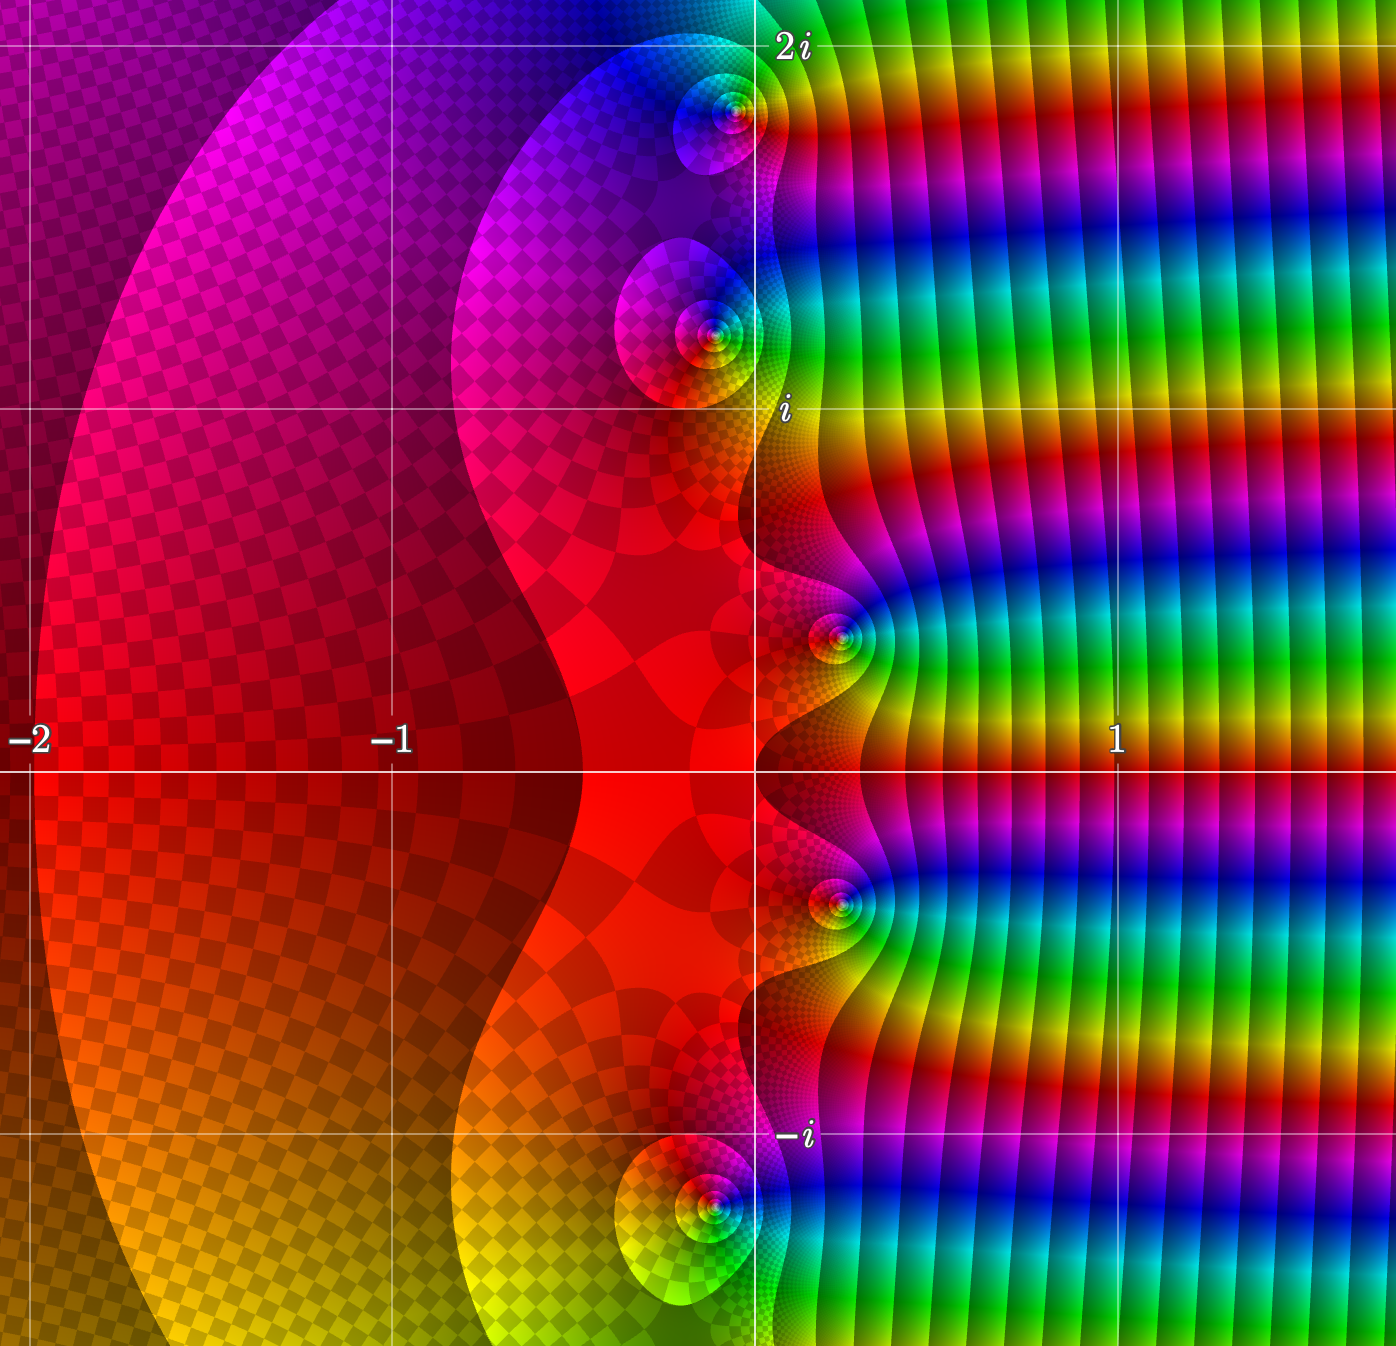
\includegraphics[scale=0.5]{img/domain.png}}; 
\end{scope}
\end{tikzpicture} 
\end{center}
\section{Consequences}

\chapter{Baker's Theorem}
\begin{mybox}
    \theorem{(Baker's Theorem) Let $\mathbb{L} = \left\{\lambda \in \C : e^{\lambda} \in \overline{\Q}\right\}$. Then, if \[\lambda_1, \ldots, \lambda_n \in \mathbb{L}\] are linearly independent over $\Q$, }
\end{mybox}
\chapter{Schanuel's Conjecture}
\begin{mybox}
    \conjecture{(Schanuel's Conjecture) Suppose we have $n$ complex numbers \[z_1, \ldots, z_n\] that are linearly independent over $\Q$. Then, $\Q(z_1, \ldots, z_n, e^{z_1}, \ldots, e^{z_n})$ has transcendence degree at least $n$ over $\Q$.} 
\end{mybox}

\backmatter{}
\printindex
\newpage{}
\end{document}
